\section{图像外观}
\label{sec:plot-appearance}

图~\ref{fig:plot-appearance}~展示了一个标准的SAC图像所包含的元素。

\begin{figure}[H]
\centering
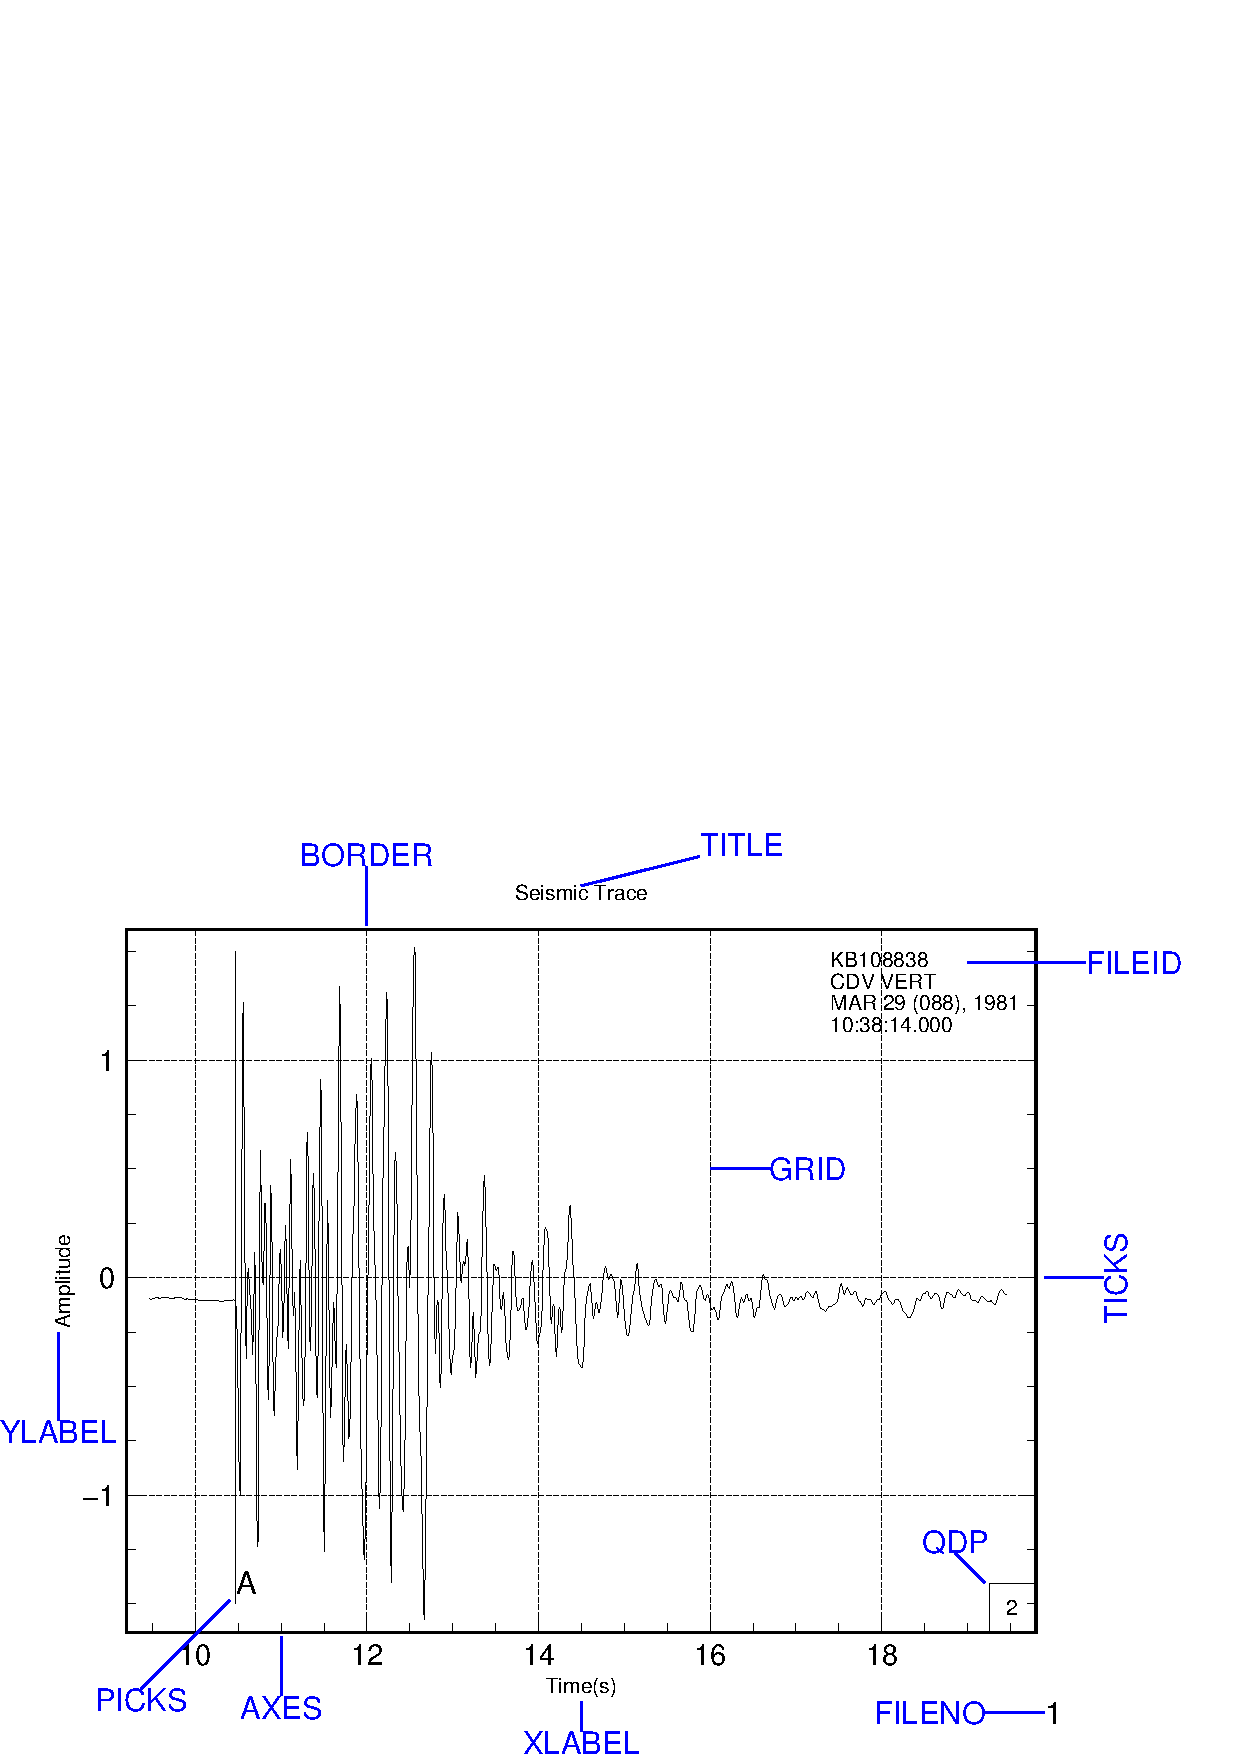
\includegraphics[width=0.9\textwidth]{appearance}
\caption[绘图外观相关命令]{绘图外观及其相关命令。图中蓝色部分为对绘图外观的说明。}
\label{fig:plot-appearance}
\end{figure}

图~\ref{fig:plot-appearance}~可以用如下命令绘制得到:
\begin{SACCode}
SAC> fg seis                // 生成数据
SAC> grid on                // 显示网格                                          
SAC> title 'Seismic Trace'  // 设置标题                                          
SAC> xlabel "Time(s)"       // 设置x轴标签                                          
SAC> ylabel "Amplitude"     // 设置y轴标签                                       
SAC> filenumber on          // 显示文件号                                       
SAC> axes only left bottom  // left和bottom显示axes
SAC> ticks only right       // right显示ticks    
SAC> border on              // top显示border                                     
SAC> p                      // 绘图
\end{SACCode}

与之相关的命令列举如下:
\begin{description}
\item [fileid] 控制文件id的显示效果(右上角FILEID)
\item [filenumber] 控制文件号的显示(图右下角FILENO)
\item [picks] 控制时间标记的显示效果(图左侧PICKS)
\item [title] 指定标题及其属性(图上部TITLE)
\item [plabel] 通用标签,相比xlabel和ylabel更加灵活
\item [grid] 控制网格的显示以及网格的线型
\item [gtext] 控制绘图文本的字体及字号
\item [tsize] SAC自定义了四种文本大小,分别为tiny、small、medium和large,
    此命令可以修改其代表的具体文本大小值
\end{description}

图中右下角的``2''称之为``qdp因子'',qdp的全称是``quick and dirty plot''。在SAC开发
的早期,计算机的性能一般,若数据点数过多,绘图会耗费大量时间,因而SAC采用了``qdp''
的方式,每隔若干个数据点绘制一个数据点。目前计算机的性能已经足以同时绘制所有数据点,
因而一般关闭qdp,可以使用~\lstinline{qdp off}~命令。

每个绘图都有一个边框,每个边框有上下左右四个边。按照标准的说法,图\ref{fig:plot-appearance}
中,上边为``border'',右边为``border+ticks'',左边和下边为``border+ticks+annotations''。

SAC对于边的定义稍有不同,其将左边和下边称之为``axes'',右边称之为``ticks'',上边
称之为``border''。用axes命令可以控制在哪些边使用``axes'',只有不使用``axes''的边
才可以用ticks命令控制是否使用``ticks'',而只有不使用``axes''和``ticks''的边才可以使用
border命令控制是否使用``border''。

有一些命令可以分别针对X和Y轴进行设置,下面仅列出与X轴相关的命令:
\begin{description}
\item [xlabel] 控制X轴标签
\item [xlim] 控制X轴范围
\item [xdiv] 控制X轴注释的间隔
\item [xgrid] 控制X轴网格的显示
\item [xfudge] 设置fudge因子以控制X轴范围
\end{description}

在绘制时间序列时一般都使用线性坐标,SAC也提供了一堆命令以控制X、Y轴是线性坐标
还是对数坐标。这些命令包括: \nameref{cmd:linlin}、\nameref{cmd:linlog}、\nameref{cmd:loglin}、
\nameref{cmd:loglog}、\nameref{cmd:xlin}、\nameref{cmd:xlog}、\nameref{cmd:ylin}、\nameref{cmd:ylog}。

对于对数坐标,还有一些命令可以控制其外观,比如\nameref{cmd:xfull}、\nameref{cmd:loglab}、
\nameref{cmd:floor}。

对于等值线图(即3D数据)而言,还有命令\nameref{cmd:zcolors}、\nameref{cmd:zlabels}、
\nameref{cmd:zlevels}、\nameref{cmd:zlines}、\nameref{cmd:zticks}。
